\subsection{Replication With Frozen Predictors}
\label{app:restoration-replication}

We generated another 15 scenario blocks with the design of the preceding
experiment. Each block shares the initial disturbance, the PMU noise and
the reports up to a possible second onset among its paired arms. Initial
and second interventions have disjoint active intervals. Their
electromechanical responses can overlap. This design permits 15
independent block draws for uncertainty estimation. The 465 records
contain 420 interventions and 165 quiet records, with 1.05 hours of
quiet monitoring after startup. We use the first unassigned detection
in the inclusive interval from onset through report 45 after onset.
Each subsequent unmatched alarm counts as an extra, including a
duplicate on a disturbed record.

A separate development check tested the integration of generator
torque amplitude. We kept the physical responses, pulse durations,
priors and alarm threshold fixed and replaced three Gauss--Legendre
nodes with seven over the same amplitude interval. On six development
blocks both rules correctly identified 154 of 168 family--asset pairs
within the deadline and 146 before clearance. Each issued two unmatched
alarms. Seven nodes advanced three correct declarations at bus~37 by
0.1~s. No event gained or lost a timely diagnosis, so we retained the
three-node rule.

\paragraph{Checking the physical continuation.}
An apparent second event can be a mismatch in the recovery fit. For
a proposed fault, line or load after the first physical fit, we
compared the observed complex voltages with the fitted continuation
$V_{0,p}(j)$ and with a forecast $V_{1,p}(j)$ that also includes the
proposed change. Both use only reports through the decision time $k$.
The forecast combines departures in log magnitude and phase relative to
the same quiet voltage. A candidate load of relative strength $a$
adds $\overline{0.1\,aS_b}/|V_{b,0}|^2$ to the bus diagonal of the
admittance matrix, where $S_b$ is its base complex load. Over the
available reports from the fitted onset $u$ through $k$, write
\[
 E_i=\sum_{j=u}^k\sum_{p=1}^{8}
         |V^{\rm obs}_{p}(j)-V_{i,p}(j)|^2 .
\]
With independent circular complex Gaussian errors of fixed variance,
the log likelihood gain is proportional to $E_0-E_1$. The tested rule
requires $1-E_1/E_0\geq 0.50$ before publishing the candidate and
updating the history. This relative cutoff is empirical. The same
measurements fit and assess the candidate. The rule leaves the
generator decision unchanged.

The operating point and the decision to retain the original monitor
were fixed on six development blocks. At the selected check threshold,
joint successes fell from 142 to 141 out of 168 and extras fell from
20 to 17. We kept the voltage check as a paired experimental arm.
Its blind difference from the original rule has a 95\% block-bootstrap
interval of $\RepCheckJointCI$ percentage points for joint accuracy
and $\RepCheckExtrasCI$ alarms for the total extra count. All intervals
in this replication use 12,000 paired resamples of whole blocks.
The article source includes the five streaming confusion matrices
and the joint and before-clearance counts for each block in
\texttt{restoration\_block\_counts.csv}. Row zero of each matrix
counts unmatched alarms by reported family. Column zero counts
events without a timely diagnosis.

\begin{table}[t]\centering\footnotesize
\caption{Detection and attribution before clearance in the four-family replication. Quiet extras count unmatched alarms on 165 quiet records.}
\label{tab:restoration-timing}\setlength{\tabcolsep}{3pt}
\begin{tabular*}{\columnwidth}{@{\extracolsep{\fill}}lrrr@{}}\toprule
Method & Detected & Joint while active & Quiet extras \\
\midrule
Recovery bank & 408 & 379 & 0 \\
With voltage check & 396 & 368 & 0 \\
Earlier physical bank & 397 & 379 & 0 \\
Sequential GLR & 338 & 315 & 0 \\
Refitted ExtraTrees & 306 & 108 & 0 \\
\bottomrule\end{tabular*}\end{table}


Of the 420 events in the replication, the selected bank missed 12,
assigned the wrong family to three and assigned the correct family to
the wrong asset in six. Ten misses were generator pulses and two were
loads at bus~16 following a fault. The joint accuracy was 399/420
(95.0\%), compared with 408/420 (97.1\%) in the preceding trial on the
same reserved asset catalog. The three extra alarms arose in disturbed
records, two with successive line openings and one with an isolated
fault. All five streaming methods were silent on all 165 quiet records.

\paragraph{Comparators and input data.}
The earlier physical bank retains its original detection stream and a
generator-specific recovery check. The selected bank compares all four
families against continued recovery and admits shorter torque pulses.
Both use the same odds divisor of 16. The sequential GLR takes the
largest Student log likelihood ratio
over source, recent onset and template in the original physical
signature bank. The recovery monitor instead averages over its
weighted histories and includes a fitted recovery forecast and a
short-pulse generator prior. Their comparison measures the complete
decisions. The GLR threshold of 150 was the only one of six development
values to give at most 18 total extras and zero quiet extras. At this
point the GLR made 115 joint identifications in 168 development events.
The refitted ExtraTrees monitor runs continuously on the same
raw reports. We excluded the reserved assets from labeled simulation
training and development. The archived forest has its original fitted
weights and decision interface. Its fitted, family-specific location
class lists contained the true asset in all 72 isolated events in the
30-s test. The archived system called only three of those windows
abnormal, including two with the correct family. Most losses thus
occurred before localization. The archived model card reports a
macro-F1 of 0.9598 and exact localization of 0.8524 on its own
simulation benchmark. Those figures and the window-close results here
come from different event distributions and scoring protocols.

CNN-F and MultiRocket-Hydra received 100 training windows per target
family. CNN-F selected its weights on 30 further cases per family.
Within each family, training and validation used separate target
assets. A bus could appear in another family across these two sets.
The final test assets were excluded across all four families. Each
target followed a restored load or line. Weak faults and short generator pulses were
included. Training trigger delays were drawn from development. The
spectral classifier uses dynamic mode decomposition to extrapolate the
preceding disturbance when subtraction is enabled. MultiRocket-Hydra
uses 60 reports from $b-30$ through $b+29$ for an alarm at $b$,
31 PMU coordinates normalized on training data, and the default
classifier in \texttt{aeon} 1.6.0. The 95\% paired intervals for the
bank's difference in timely family accuracy are $\RepCnnCI$
percentage points against CNN-F and $\RepHydraCI$ against
MultiRocket-Hydra. Neither learned classifier supplies the alarm
or the asset in this comparison. On the 120 development validation
cases, CNN-F with and without subtraction classified 81 and 75
correctly. MultiRocket-Hydra classified 106 correctly. The blind
second events followed faults or line openings. This change in the
preceding event distribution limits what the test establishes about
the learned classifiers on other sequences.

The archived system receives balanced three-phase reports reconstructed
from positive-sequence voltage and current. A causal phase fit supplies
frequency and its rate of change. The four-family macro-F1 gives equal
weight to bus faults, line openings, positive torque pulses and load
changes. In addition to the native 30-s comparison, we used the last
partial window allowed by the archived implementation. At 24~s the bank
and archived trees identified the family on \RepBankPartialFamily{}
and \RepArchPartialFamily{} of 180 isolated events. They identified
both family and asset on \RepBankPartialJoint{} and
\RepArchPartialJoint{} and flagged \RepBankPartialQuiet{} and
\RepArchPartialQuiet{} of 165 quiet records. The common deadline in
these two window experiments was record close. The streaming
deadline applies only to the continuous tests.

\paragraph{Recovery alignment at a known onset.}
We evaluated the mean-shift identity from the main article on the six
nominal development blocks. Each sequence had paired quiet, first-event
only and two-event records with the same noise. We passed all three
through the fixed nominal innovation filter. For the first 30 reports
after the known second onset, subtracting quiet from the first-event
record gave $d$. Subtracting the first-event record from the two-event
record gave $s$. In these whitened coordinates the ratio
$s^\top d/(s^\top s)$ measures the signed shift in log evidence from
dropping the recovery mean, relative to the energy of the proposed
switch. Its median was $-0.540$ for a generator pulse following a fault,
$0.026$ for a load following a fault, $0.075$ for a generator pulse
following a line opening, and $0.011$ for a second line opening.
One of 24 pairs exceeded $0.5$, a generator pulse after a line opening.
Figure~\ref{fig:restoration-alignment} shows the individual pairs.
The same recovery can mask or mimic a new intervention depending on
its measured direction. This retrospective calculation uses the known
onset and paired counterfactual reports. It serves to interpret the
filter and contributed no decision variable at test time.

\begin{figure}[t]\centering
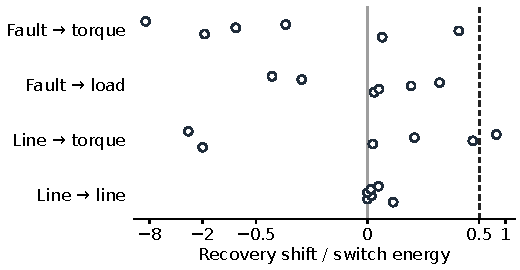
\includegraphics[width=.96\columnwidth]{figures/generated/restoration_alignment.pdf}
\caption{Shift in the Gaussian log likelihood ratio from dropping
the mean recovery trajectory, divided by the second switch's energy.
Each row contains the six nominal development blocks. The dashed line
marks the value above which a reset favors the proposed switch on
average under recovery alone. The horizontal scale is linear near zero
and logarithmic in the tails.}
\label{fig:restoration-alignment}
\end{figure}
